\section{外部性的量级与结构}\label{sec:magnitude}

本节是全文最硬的部分，因为它完全不依赖政策变异。

\subsection{尖峰的位置与量级}

图~\ref{fig:event} 给出春节窗口内日均 \pmm{2.5} 的事件研究剖面。作图使用 308 城的作图画板，\textbf{只取 2015—2019 与 2022—2026 两个年代}；每个年代每个相对日的样本量约为 $1{,}540$（308 城 $\times$ 5 年）。\textbf{注意：全样本的 63,515 个城市-日属于 389 城面板，不用于这张图。}峰值出现在\textbf{正月初一}，随后快速回落。图~\ref{fig:event}(b) 给出四种污染物的指数化剖面（以 \texttt{rel\_day} $=-7$ 为 100）。

\begin{figure}[H]
\centering
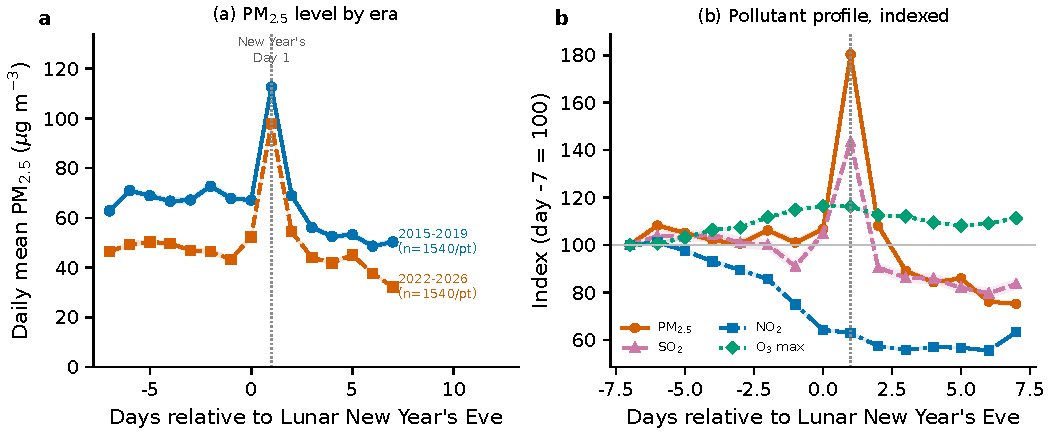
\includegraphics[width=\textwidth]{fig1_event_study.pdf}
\caption{春节窗口的事件研究剖面。(a) 各城市在除夕前 7 日至后 7 日的日均 \pmm{2.5}，按 2015—2019 与 2022—2026 两个年代分别取均值，阴影为 $\pm 1$ 标准误；(b) 四种污染物在同一窗口内的指数化剖面，以除夕前 7 日 $=100$。竖虚线标出正月初一。}
\label{fig:event}
\end{figure}

尖峰增量的分布如下表。两个样本口径都列出，理由见第~\ref{sec:panel}~节。

\begin{table}[H]
\centering
\caption{正月初一尖峰增量（初一 $-$ 节前基线）的分布}
\label{tab:spike-dist}
\small
\begin{tabular}{L{4.0cm}R{2.3cm}R{2.3cm}R{2.3cm}R{2.3cm}}
\toprule
\textbf{样本} & \textbf{城市-年} & \textbf{均值} & \textbf{中位数} & \textbf{标准差} \\
\midrule
平衡面板（估计口径） & 3,672 & 43.1 & 28.1 & 67.7 \\
非平衡面板（描述口径） & 4,240 & 40.0 & 24.8 & 66.0 \\
\bottomrule
\end{tabular}
\end{table}

平衡面板上，尖峰增量的分位数为：$p_{10}=-21.7$、$p_{25}=1.6$、$p_{50}=28.1$、$p_{75}=71.8$、$p_{90}=126.3$、$p_{99}=273.8$，最大值 440.9。\textbf{23.3\% 的城市-年尖峰增量为负}，即当年初一反而比节前基线更干净；15.7\% 的城市-年增量超过 100 \ugm。

均值与中位数的差距本身就说明问题：\textbf{分布是右偏的}。少数城市有巨尖峰，多数城市的中位增量不到 30 \ugm。这一点在后文有直接后果——任何假设“统一处理效应”的设计都会在量级上先出问题。

\subsection{城际异质性}

图~\ref{fig:hetero} 把 308 个城市的基线浓度与尖峰幅度作图。两个事实值得记录。

第一，\textbf{基线越高，相对倍数越低}（图~\ref{fig:hetero}a）。这其中有相当部分是分母效应：以基线为分母时，低基线城市天然倍数大。\textbf{因此相对倍数不适合作为跨城比较的主口径。}

第二，\textbf{绝对增量的城际差异极大}（图~\ref{fig:hetero}b）。以上海为例：12 年平均为 $-2.5$ \ugm，但逐年值从 $-68.0$（2020）到 $+144.2$（2024）——\textbf{平均值掩盖了 2024 年的大尖峰}。因此既不能说“春节一定有尖峰”，也不能因为一个城市的均值接近零就判定它没有尖峰；\textbf{均值不是可以替代逐年观察的统计量。}

\begin{figure}[H]
\centering
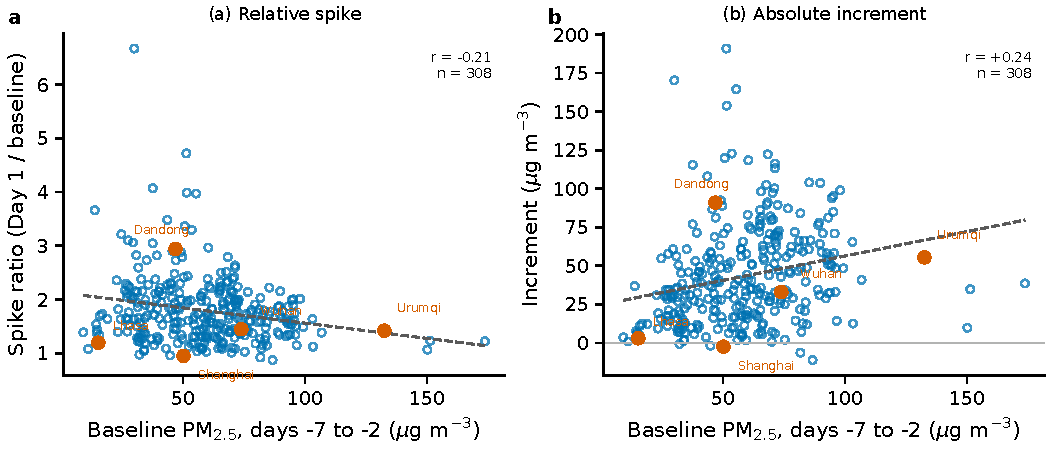
\includegraphics[width=\textwidth]{fig3_heterogeneity.pdf}
\caption{308 个平衡面板城市的尖峰幅度与基线浓度。(a) 相对倍数（峰值／基线）对基线浓度；(b) 绝对增量（峰值 $-$ 基线）对基线浓度。虚线为最小二乘拟合线，橙色点标注五座城市（武汉、丹东、上海、乌鲁木齐、拉萨）。注：图 (a) 的纵轴以基线为分母，负相关中有相当部分是分母效应。}
\label{fig:hetero}
\end{figure}

\subsection{机制证据}

图~\ref{fig:event}(b) 的污染物结构提供了机制线索：

\begin{itemize}
  \item \textbf{\SOtwo{} 与 \pmm{2.5} 在正月初一同步抬升}。烟花爆竹配方含硫，这一同向性是燃放的特征。
  \item \textbf{\NOtwo{} 在整个窗口内单调下降}，初一无跳变。
  \item \textbf{\Othree{} 日最大值仅随日照变长缓慢上升}，初一无跳变。
\end{itemize}

图~\ref{fig:hourly} 给出五座城市除夕 12:00 至初一 06:00 的逐小时曲线。跨零点的爆发在各城形态一致、幅度差异极大：这既确认了尖峰的时间位置，也说明\textbf{用日均值衡量会把一个数小时的尖峰摊薄}——第一节所说的“口径决定结论”，在这里可以直观看到。

\begin{figure}[H]
\centering
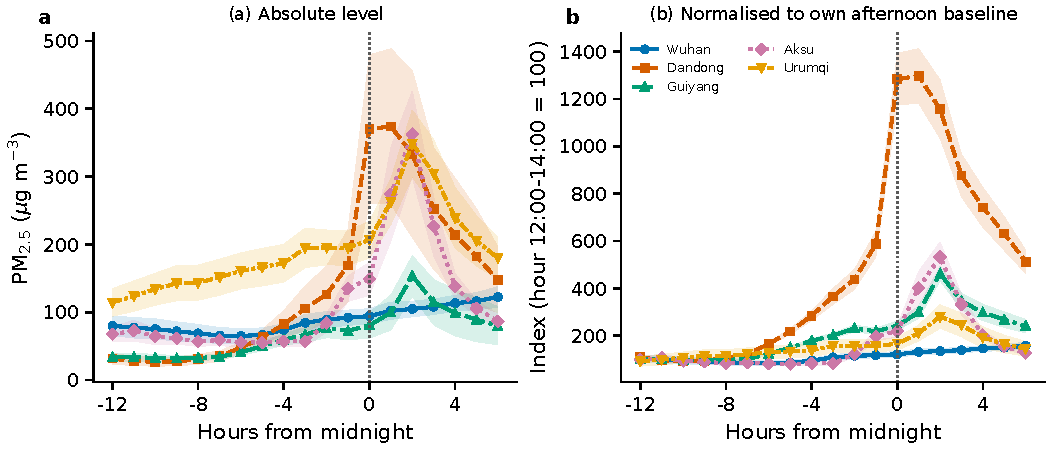
\includegraphics[width=0.92\textwidth]{fig2_hourly.pdf}
\caption{除夕午后至初一清晨的逐小时 \pmm{2.5}（五城，跨 12 个春节窗口取平均）。(a) 绝对水平（\ugm）；(b) 按各自除夕 12:00—14:00 的均值归一化为 100。阴影为 $\pm 1$ 标准误（$n=12$ 年）。注：本图基线取小时值，显示的倍数显著大于日均口径，两者不可直接比较。}
\label{fig:hourly}
\end{figure}

这里有一处必须写准的地方。\textbf{\NOtwo{} 的下降是假期效应，不是“没有交通源”的证据。} Jiang et al.（2015）已证明春节假期使北京 NO 下降约 54\%，主要来自停驶停产。本文的论证因此不能写成“\NOtwo{} 没升所以不是交通”，而应写成：

\begin{quote}
\SOtwo{} 与 \pmm{2.5} 同向上升，而 \NOtwo{} 因假期效应下降——\textbf{两者方向相反，恰好说明尖峰不是由交通驱动的}。若尖峰由交通造成，\NOtwo{} 应当与 \pmm{2.5} 同向上升。
\end{quote}

这个逻辑成立，且比原表述更难被驳倒。

\subsection{与既有文献的口径分歧}

既有文献对“禁放有没有效”给出的数字相差一个数量级，而分歧几乎全部来自\textbf{口径}：

\begin{table}[H]
\centering
\caption{春节污染与禁放效应的既有估计：估计对象并不相同}
\label{tab:caliber}
\small
\begin{tabular}{L{3.0cm}L{3.2cm}L{4.0cm}L{3.4cm}}
\toprule
\textbf{估计对象} & \textbf{窗口口径} & \textbf{结论} & \textbf{出处} \\
\midrule
春节效应（非禁放） & 初一日均 & 原始效应 $+89\%$ & Li et al.（2025） \\
春节效应（非禁放） & 春节窗口均值 & 为平均值的 159\%—223\% & Zhang et al.（2020） \\
春节效应（非禁放） & 年度均值 & 仅约 6.4\% & 陈欣等（2014） \\
\midrule
\textbf{禁放效应} & 小时峰值 & 显著压低（$-32.2\%$） & 陆卜梵、刘蓓蓓（2022） \\
\bottomrule
\end{tabular}

\vspace{0.3em}
{\small 注：前三行估计的是“春节本身抬高了多少”，最后一行估计的是“禁放压低了多少”，两者不是同一个 estimand。把它们并排比较会得出错误的“口径分歧”结论；本表保留这种并排，正是为了说明文献中常被混淆的一点。}
\end{table}

\textbf{同一现象，估计对象与窗口一变，量级差一个数量级。} 这构成本文的一条方法论主张：\textbf{“禁放有没有效”这个问题，在给定口径之前没有答案。}

一处张力：Chen et al.（2022）报告节庆月 \pmm{2.5} 下降 8\%，而一次持续一天的尖峰对月均值最多贡献约 2\%。这个差距提示两文的变量口径不同。\textbf{本文只把它作为待问的问题，不写成反驳}——没有读到其处理变量与结果变量的逐字定义。

\subsection{变异的分解：工具够不到的是哪一部分}\label{sec:variance}

第~\ref{sec:resolution}~节把解析度写成了 $L(\mathcal{P})=\sigma^2-\operatorname{Var}(\mathbb{E}[D\mid\text{cell}])$。在平衡面板（306 城 $\times$ 12 年 $=3{,}672$ 个城市-年）上，对尖峰增量做双向方差分解，可以得到三个可以直接代入的百分比：

\begin{table}[H]
\centering
\caption{尖峰增量的方差分解（平衡面板，$N=3{,}672$）}
\label{tab:variance}
\small
\begin{tabular}{L{6.8cm}R{3.0cm}R{4.2cm}}
\toprule
\textbf{变异来源} & \textbf{占总平方和} & \textbf{对应的工具划分} \\
\midrule
城市间（同一城市跨年不变的部分） & 22.0\% & 按城市设定的税率 \\
年份间（全国共同趋势） & 12.7\% & 按年调整的全国税率 \\
城市 $\times$ 年份残差 & \textbf{65.3\%} & 只有城市 $\times$ 时段工具能够触及 \\
\midrule
合计 & 100\% & \\
\bottomrule
\end{tabular}

\vspace{0.3em}
{\small 注：被分解的变量为正月初一尖峰增量（初一减节前基线，\ugm），样本为 306 城 $\times$ 12 年 $=3{,}672$ 个城市-年。城市间与年份间为单向平方和，残差为总平方和减去二者之和（平衡面板下可加）。三个百分比之和为 100\%。}
\end{table}

换成第~\ref{sec:resolution}~节的语言：一个全国统一、按年适用的从价税只有一个格子，$L$ 等于总方差；即便把税率按城市设定（仍由中央统一），$L$ 也只降到总方差的 78\%；而\textbf{三分之二的变异落在“哪个城市、哪一年”这个交点上，任何不随城市与年份变化的工具在构造上都够不到它}。

这个结果有三处必须说明的限制。第一，它分解的是\textbf{已实现}的尖峰增量，其中包含当日气象等不可预测成分；工具能利用的只是可预期部分，因此 65.3\% 应读作\textbf{“分辨率缺口的量级”}，不是可实现福利损失的估计。第二，它按年度频率分解，未涉及小时维度；而燃放损害在小时上的集中程度远高于年度。第三，方差分解本身不回答“应不应该用数量工具”，那是第~\ref{sec:theory}~节 Weitzman 条件的问题。

尽管有这些限制，这张表完成了本文想做的一件小事：\textbf{把“工具形式不对准”从一句判断，变成一个可以被别人用同一份数据重算的三个数。}
